\documentclass[11pt,a4paper]{article}

\usepackage[margin=1in]{geometry}
\usepackage{booktabs}
\usepackage{enumitem}
\usepackage{hyperref}
\usepackage{amsmath}
\usepackage{float}
\usepackage{setspace}
\usepackage{tikz} 
\usetikzlibrary{shapes.geometric, arrows.meta, positioning, calc, backgrounds}

\setstretch{1.15} 

\title{\textbf{ML-Based Flood Prediction System Using Historical Threat Mapping and Live Weather APIs}}

\author{
    \textbf{Submitted to: Dr. Jeelani} \\[0.5cm]
    Amit Bishnoi (1024240005) \\
    Diksha Garg (1024240015) \\[0.5cm]
    Thapar Institute of Engineering and Technology
}
\date{August 2026}

\begin{document}

\maketitle

\section{Introduction \& Problem Statement}
Floods cause massive damage around the world. Because of climate change, they are happening more often, making it crucial to have better ways to predict them. Right now, weather apps show us live data like rain and wind, but they do not tell us if that rain will actually cause a flood in a specific area. 

On the other hand, traditional flood maps are usually drawn once and rarely updated. They cannot react to a sudden, heavy storm. Also, databases that track past disasters (like EM-DAT) have great details on the damage caused, but they often lack exact GPS coordinates. Because of this, current systems struggle to instantly connect a live storm with a location's history of flooding.

Our project aims to fix this gap. We are building a system that takes live weather data and compares it against a combined database of past floods. By merging the exact GPS data from the Dartmouth Flood Observatory (DFO) with the impact records from EM-DAT, our machine learning model will be able to predict the real-time flood risk for any searched location.

\section{Literature Review}
Past flood prediction relied heavily on complex physical models of rivers and terrain, which require immense computing power and are difficult to scale for smaller cities. While Machine Learning (ML) has emerged as a faster alternative to predict water levels, current systems largely fail to integrate live weather API data with long-term disaster records. This project bridges that gap by treating geographic vulnerability as dynamic, mixing real-time weather conditions with historical data to calculate an instant, automated risk score.

\section{Objectives}
The main goal of this project is to build a machine learning system that uses live weather data and past disaster records to predict current flood risks.

Specific steps to achieve this include:
\begin{itemize}[noitemsep]
    \item To pull real-time weather data (like rainfall, temperature, and wind speed) using the OpenWeatherMap API.
    \item To clean and combine the EM-DAT and DFO datasets to create a complete history of floods with exact GPS coordinates.
    \item To create custom data features for our model, such as past flood severity and how much it rained in the last 48 hours.
    \item To train and test machine learning models to predict if the flood risk is Low, Medium, or High.
    \item To build a simple user interface where anyone can search a location and see its live weather and risk score.
\end{itemize}

\section{Methodology \& System Architecture}
The project relies on a five-stage data pipeline, taking raw live signals and turning them into a final risk score. The overall system architecture is illustrated in Figure \ref{fig:architecture}.

\begin{figure}[H]
    \centering
    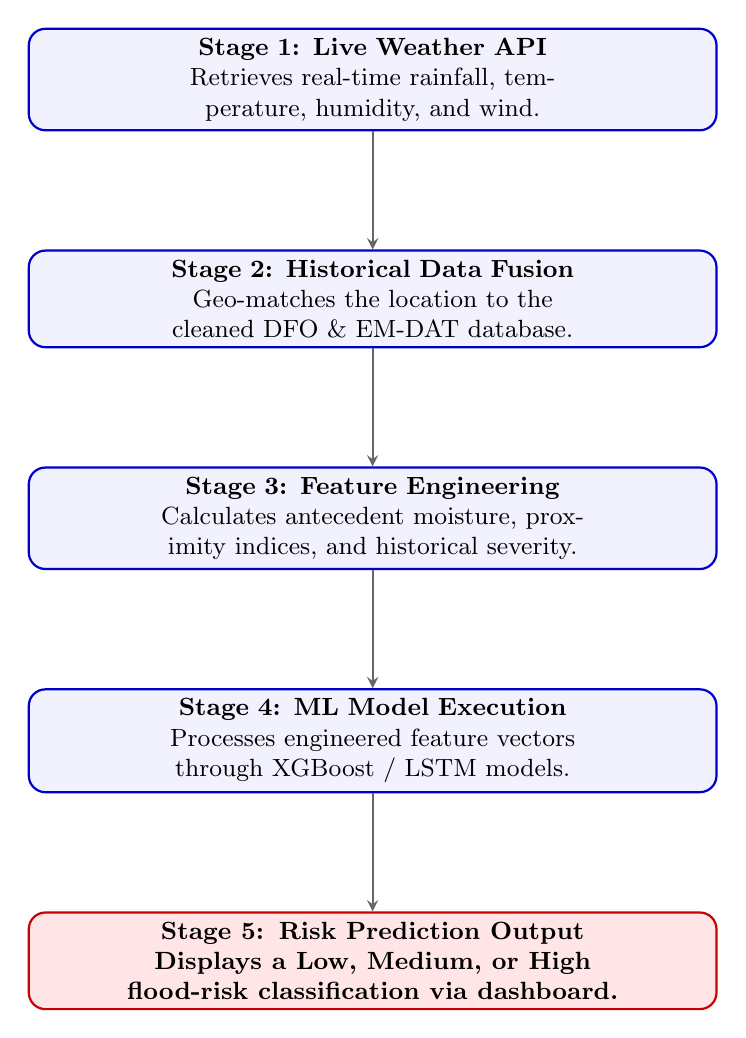
\begin{tikzpicture}[
        node distance=1.5cm and 1cm,
        stageBlock/.style={
            rectangle, rounded corners=6pt, draw=blue!80!black, thick,
            fill=blue!5, text width=8.5cm, text centered, minimum height=1.1cm,
            font=\small
        },
        finalBlock/.style={
            rectangle, rounded corners=6pt, draw=red!80!black, thick,
            fill=red!10, text width=8.5cm, text centered, minimum height=1.1cm,
            font=\small\bfseries
        },
        arrow/.style={
            thick, ->, >=stealth, draw=gray!80!black
        }
    ]
        % Nodes
        \node (stage1) [stageBlock] {\textbf{Stage 1: Live Weather API} \\ Retrieves real-time rainfall, temperature, humidity, and wind.};
        \node (stage2) [stageBlock, below=of stage1] {\textbf{Stage 2: Historical Data Fusion} \\ Geo-matches the location to the cleaned DFO \& EM-DAT database.};
        \node (stage3) [stageBlock, below=of stage2] {\textbf{Stage 3: Feature Engineering} \\ Calculates antecedent moisture, proximity indices, and historical severity.};
        \node (stage4) [stageBlock, below=of stage3] {\textbf{Stage 4: ML Model Execution} \\ Processes engineered feature vectors through XGBoost / LSTM models.};
        \node (stage5) [finalBlock, below=of stage4] {\textbf{Stage 5: Risk Prediction Output} \\ Displays a Low, Medium, or High flood-risk classification via dashboard.};

        % Arrows
        \draw [arrow] (stage1) -- (stage2);
        \draw [arrow] (stage2) -- (stage3);
        \draw [arrow] (stage3) -- (stage4);
        \draw [arrow] (stage4) -- (stage5);
    \end{tikzpicture}
    \caption{System Architecture: End-to-end data pipeline from live signal to classified risk score.}
    \label{fig:architecture}
    
\end{figure}

\subsection{Stage 1: Live Weather API}
The system starts by searching a specific location. It pulls real-time rainfall, temperature, humidity, and wind speed for that exact spot using the OpenWeatherMap REST API.

\subsection{Stage 2: Historical Data Fusion}
The historical data pipeline addresses the spatial limitation of EM-DAT by merging it with DFO centroids, as illustrated in Figure \ref{fig:data_fusion}. We clean and filter historical flood events using our fused database, geo-matching past events to the user's searched coordinates.

\begin{figure}[H]
    \centering
    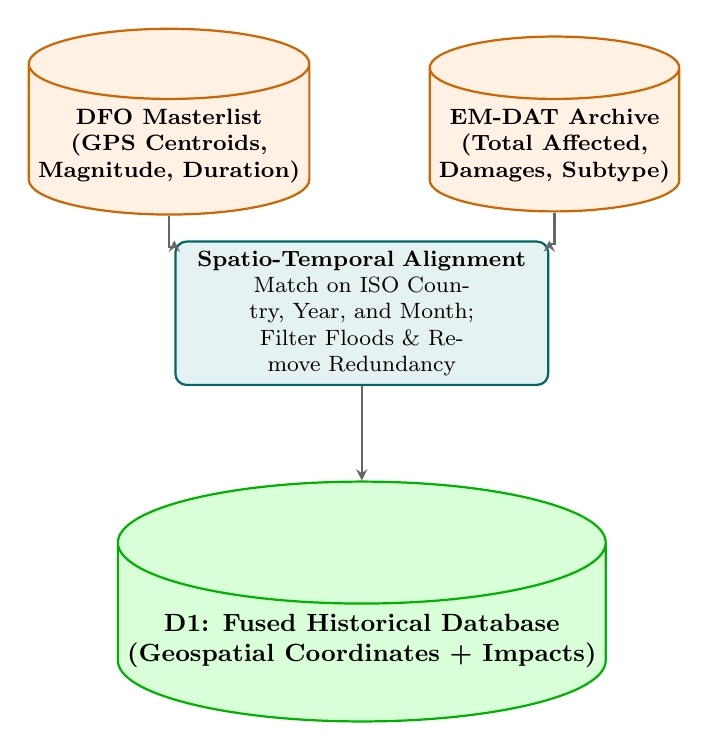
\begin{tikzpicture}[
        node distance=1.2cm and 1.5cm,
        dbNode/.style={
            cylinder, shape border rotate=90, draw=orange!80!black, thick,
            fill=orange!10, aspect=0.25, minimum width=2.8cm, minimum height=1.3cm,
            font=\footnotesize\bfseries, align=center
        },
        procNode/.style={
            rectangle, rounded corners=4pt, draw=teal!80!black, thick,
            fill=teal!10, text width=4.5cm, text centered, minimum height=1.2cm,
            font=\footnotesize
        },
        fusedNode/.style={
            cylinder, shape border rotate=90, draw=green!70!black, thick,
            fill=green!15, aspect=0.25, minimum width=3.4cm, minimum height=1.4cm,
            font=\small\bfseries, align=center
        },
        arrow/.style={
            thick, ->, >=stealth, draw=gray!80!black
        }
    ]
        % Source nodes
        \node (dfo) [dbNode] {DFO Masterlist\\(GPS Centroids,\\Magnitude, Duration)};
        \node (emdat) [dbNode, right=of dfo] {EM-DAT Archive\\(Total Affected,\\Damages, Subtype)};
        
        % Fusion process
        \node (align) [procNode, below=1.2cm of $(dfo)!0.5!(emdat)$] {
            \textbf{Spatio-Temporal Alignment}\\
            Match on ISO Country, Year, and Month; \\ Filter Floods \& Remove Redundancy
        };
        
        % Output fused database
        \node (fused) [fusedNode, below=1.2cm of align] {
            D1: Fused Historical Database\\(Geospatial Coordinates + Impacts)
        };

        \draw [arrow] (dfo.south) -- ++(0,-0.4) -| (align.north west);
        \draw [arrow] (emdat.south) -- ++(0,-0.4) -| (align.north east);
        \draw [arrow] (align.south) -- (fused.north);
    \end{tikzpicture}
    \caption{Dual-Dataset Fusion Workflow: Integrating spatial resolution with impact severity.}
    \label{fig:data_fusion}
\end{figure}

\subsection{Stage 3: Feature Engineering}
In this stage, raw parameters are transformed into normalized numerical vectors. This includes calculating the spatial proximity index (using the Haversine distance to historical flood centroids), antecedent moisture metrics, and multi-hour cumulative precipitation.

\subsection{Stage 4: ML Model Training}
The processed vectors are fed into machine learning classifiers to predict risk categories:
\begin{itemize}[noitemsep]
    \item \textbf{XGBoost / Random Forest:} Best suited for tabular tabular feature vectors, yielding calibrated multi-class probabilities (Low, Medium, High).
    \item \textbf{LSTM Networks:} Evaluated for multi-step temporal dependencies where continuous sequential rainfall forecasts are available.
\end{itemize}

\subsection{Stage 5: Risk Prediction Output}
The platform aggregates the probability scores, establishes confidence intervals, and renders a localized threat level alongside live weather cards on an interactive Streamlit dashboard.

\section{Evaluation Criteria \& Validation Framework}
To ensure clinical rigor and eliminate data leakage, the model is evaluated on a partitioned 20\% holdout test set. Figure \ref{fig:evaluation_pipeline} outlines the comprehensive evaluation and metric validation protocol.

\begin{figure}[H]
    \centering
    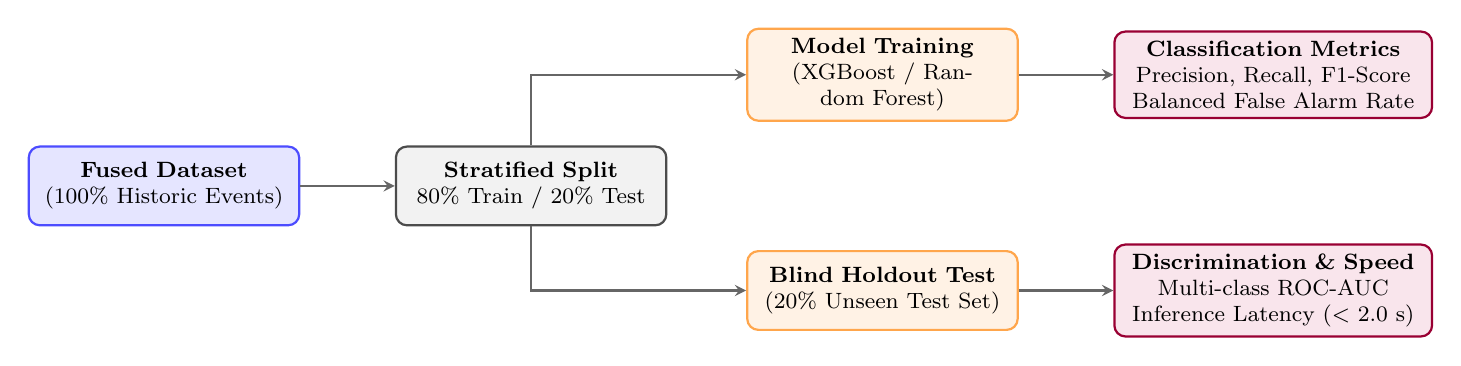
\begin{tikzpicture}[
        node distance=0.9cm and 1.2cm,
        box/.style={
            rectangle, rounded corners=4pt, draw=black!70, thick,
            fill=gray!10, text width=3.2cm, text centered, minimum height=1cm,
            font=\footnotesize
        },
        metricBox/.style={
            rectangle, rounded corners=4pt, draw=purple!80!black, thick,
            fill=purple!10, text width=3.8cm, text centered, minimum height=1cm,
            font=\footnotesize
        },
        arrow/.style={
            thick, ->, >=stealth, draw=gray!80!black
        }
    ]
        % Pipeline Nodes
        \node (dataset) [box, fill=blue!10, draw=blue!70] {\textbf{Fused Dataset}\\(100\% Historic Events)};
        \node (split) [box, right=of dataset] {\textbf{Stratified Split}\\80\% Train / 20\% Test};
        
        \node (train) [box, fill=orange!10, draw=orange!70, above right=0.3cm and 1.0cm of split] {\textbf{Model Training}\\(XGBoost / Random Forest)};
        \node (eval) [box, fill=orange!10, draw=orange!70, below right=0.3cm and 1.0cm of split] {\textbf{Blind Holdout Test}\\(20\% Unseen Test Set)};

        % Metrics Nodes
        \node (metric1) [metricBox, right=1.2cm of train] {\textbf{Classification Metrics}\\Precision, Recall, F1-Score\\Balanced False Alarm Rate};
        \node (metric2) [metricBox, right=1.2cm of eval] {\textbf{Discrimination \& Speed}\\Multi-class ROC-AUC\\Inference Latency ($< 2.0\text{ s}$)};

        % Connectors
        \draw [arrow] (dataset) -- (split);
        \draw [arrow] (split) |- (train);
        \draw [arrow] (split) |- (eval);
        \draw [arrow] (train) -- (metric1);
        \draw [arrow] (eval) -- (metric2);
    \end{tikzpicture}
    \caption{Model Evaluation Protocol: Stratified holdout validation, multi-class assessment, and system latency benchmarking.}
    \label{fig:evaluation_pipeline}
\end{figure}

The specific performance metrics include:
\begin{itemize}[noitemsep]
    \item \textbf{Precision, Recall, and F1-Score:} Critical for balancing false alarms (false positives) against missed emergency warnings (false negatives).
    \item \textbf{ROC-AUC:} Assesses the model's ability to discriminate between Low, Medium, and High threat thresholds across various classification cutoffs.
    \item \textbf{System Latency:} Benchmarking inference and feature engineering time to ensure the complete dashboard response is generated in under 2 seconds.
\end{itemize}

\section{Project Timeline}
\begin{table}[H]
\centering
\begin{tabular}{@{} l p{7.5cm} p{5cm} @{}}
\toprule
\textbf{Phase} & \textbf{Task Description} & \textbf{Key Deliverable} \\ \midrule
Weeks 1--3 & Read existing research, set up API keys, and clean the data. & Cleaned dataset \& working API code \\
Weeks 4--7 & Combine DFO and EM-DAT data, and start training ML models. & Trained models \& accuracy reports \\
Weeks 8--10 & Connect the backend code to the front-end user interface. & Working software prototype \\
Weeks 11--12 & Fix bugs, improve the design, and write the final report. & Final project file \& presentation \\ \bottomrule
\end{tabular}
\end{table}

\section{Resources \& Risk Assessment}
\subsection{Resources Needed}
We will use free, open-source Python libraries (like Scikit-Learn and Pandas) and public datasets (EM-DAT and DFO). The live weather data will come from the free tier of the OpenWeatherMap API. Computation will be executed on local machines with lightweight footprints, resulting in zero external budget requirements.

\subsection{Possible Risks \& Solutions}
\begin{itemize}
    \item \textbf{Mismatched Data:} When combining EM-DAT and DFO, timestamps or regional boundaries may have variance. \textit{Solution:} We employ fuzzy temporal matching (matching events within the same month/year and country) and spatial nearest-neighbor verification.
    \item \textbf{Imbalanced Data:} The dataset naturally contains fewer severe flood events than normal atmospheric days. \textit{Solution:} We utilize class weighting and Synthetic Minority Over-sampling Technique (SMOTE) to prevent majority-class bias.
    \item \textbf{API Rate Limits:} Free weather APIs enforce request frequency caps. \textit{Solution:} A local response caching store (D2) retains recent queries to avoid redundant API pings during active testing.
\end{itemize}

\section{Summary}
This project proposes a deployable, machine learning-driven platform to reduce flood-related damages by providing instant, localized risk assessments. By successfully fusing high-resolution spatial data with historical impact metrics and live weather APIs, it overcomes the severe limitations of traditional, static flood maps. The system is designed to be accessible, cost-effective, and highly scalable, offering a vital early warning tool for both everyday users and emergency responders.

\end{document}
